\documentclass[letterpaper,10pt]{article}%10 o 12 pt son recomendadas
\usepackage{graphicx} % Plantilla(s) elaboradas por Emiliano Ortega Xochihua
\usepackage{booktabs}
\usepackage{multicol}
\usepackage{import}
\usepackage{tcolorbox}
\usepackage{float}
\usepackage{amsmath}
\usepackage{amssymb}
\usepackage{lipsum}
\usepackage{nicefrac}
\usepackage{tikz}
\setlength{\parindent}{0cm}
\usepackage{geometry}
\geometry{
top=20mm,
bottom=25mm,
left=25mm,
right=25mm
}
%Para todas voy a poner el mismo contenido para ver los entornos que se recomienda usar para cualquier asignación
\begin{document}
%Plantilla 1
\colorbox{white!10!}
{
\begin{minipage}[H]{0.82\textwidth}
    \begin{flushleft}
        \LARGE{ \textbf{Tarea X (Materia)}}\\
        \vspace{0.2cm}
        \large{Profesor: Isaac Said Martínez Cerón}
    \end{flushleft}
\end{minipage}
\begin{minipage}[H]{0.15\textwidth}
    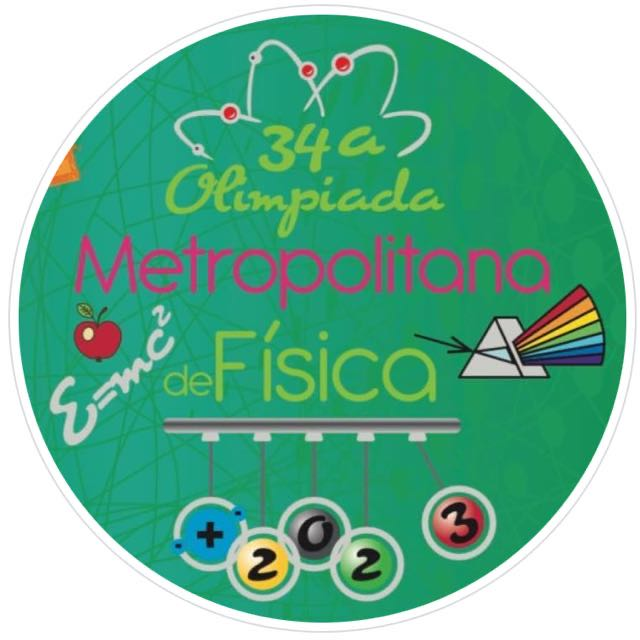
\includegraphics[width=1in]{logo34omf.jpg}
\end{minipage}
}

\begin{center}
    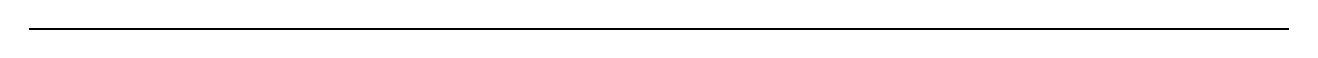
\begin{tikzpicture}
        \draw[thick] (-6.5,0)--(9.5,0);
    \end{tikzpicture}
\end{center}

\section{Preguntas y actividades}
\begin{enumerate}
    \item \textbf{Preguntas}
    Y sus respuestas
    \item \textbf{Actividades}
    Y sus respuestas
\end{enumerate}

\section{Problemas}
\begin{tcolorbox}[title=problema 1]
Descripción del problema
\end{tcolorbox}
Argumentos adecuados
\begin{equation}
    \oint formulas\,\,elementales
\end{equation}
Y más argumentos
\begin{equation*}
    \therefore\,resultado
\end{equation*}
\newpage

%Plantilla 2
\colorbox{white!10!}
{
\begin{minipage}[H]{1\textwidth}
    \begin{center}
        \begin{figure}[H]
            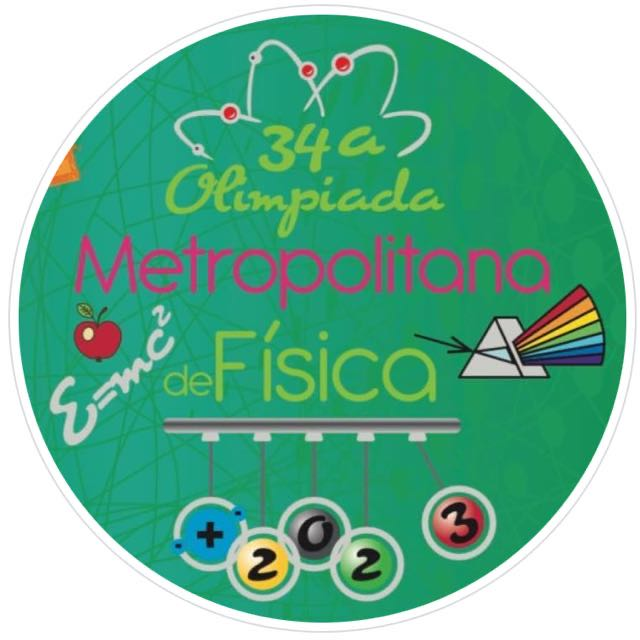
\includegraphics[height=1in]{logo34omf.jpg}
            \hfill 
            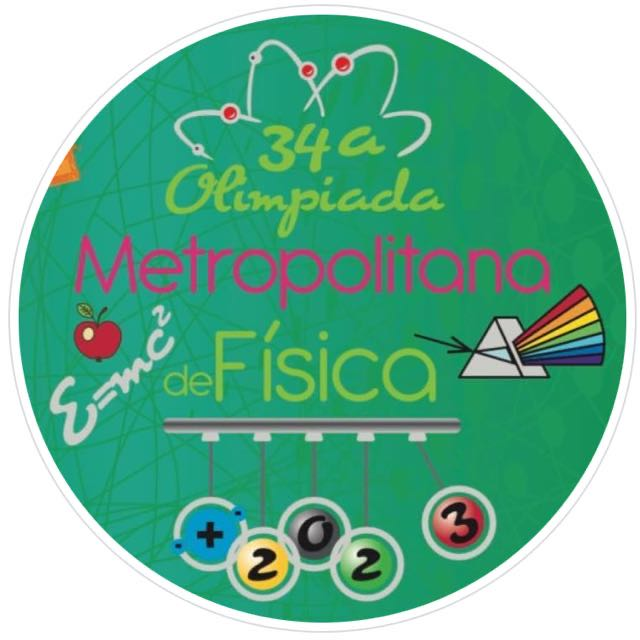
\includegraphics[height=1in]{logo34omf.jpg} 
        \end{figure}
    \end{center}
\end{minipage}
}

\vspace{3cm}
\begin{center}
    \Huge{\textbf{Tarea X (Materia)}}\\
    \vspace{2cm}
    \Large {Profesor: Isaac Said Martínez Cerón}
    \vfill
    \Large{2023}
\end{center}
\newpage

\setcounter{section}{0}
\section{Preguntas y actividades}
\begin{enumerate}
    \item \textbf{Preguntas}
    Y sus respuestas
    \item \textbf{Actividades}
    Y sus respuestas
\end{enumerate}

\section{Problemas}
\begin{tcolorbox}[title=problema 1]
Descripción del problema
\end{tcolorbox}
Argumentos adecuados
\begin{equation}
    \oint formulas\,\,elementales
\end{equation}
Y más argumentos
\begin{equation*}
    \therefore\,resultado
\end{equation*}
\newpage

%Plantilla 3
\colorbox{white!10!}
{
\begin{minipage}[H]{0.165 \textwidth}
    \begin{flushright}
        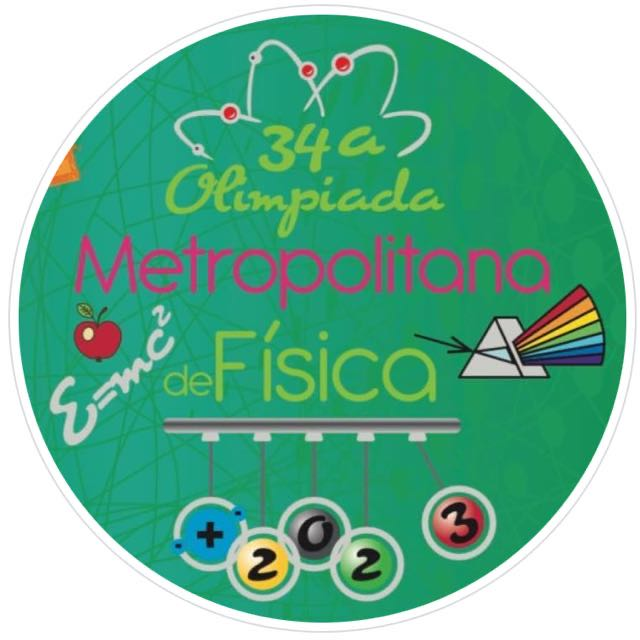
\includegraphics[width=1in]{logo34omf.jpg}
    \end{flushright}
\end{minipage}
\begin{minipage}[H]{0.62 \textwidth}
    \begin{center}
        {\vspace{1cm}
        \huge \textbf{Tarea X}}\\
        \Large Tema de la tarea e.g. magnetohidrodinámica
        \vspace{0.5cm}    
        \textbf{Profesor: Isaac Said Martínez Cerón}
        \vspace{0.5cm}
    \end{center}
\end{minipage}
\begin{minipage}[H]{0.165 \textwidth}
    \begin{flushleft}
        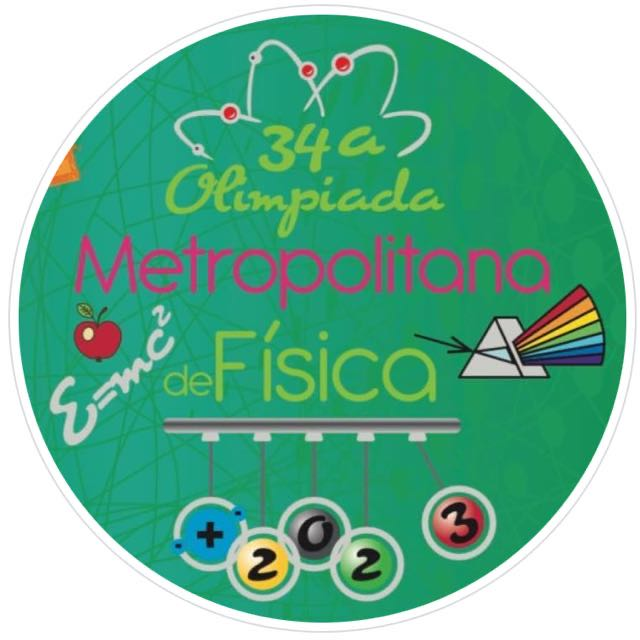
\includegraphics[width=1in]{logo34omf.jpg}
    \end{flushleft}
\end{minipage}
}

\begin{center}
    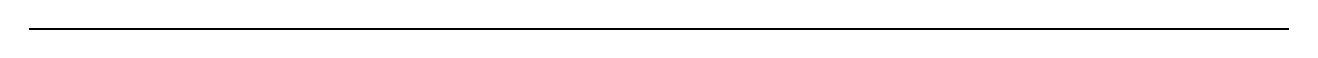
\begin{tikzpicture}
    \draw[thick] (-6.5,0)--(9.5,0);
    \end{tikzpicture}
\end{center}

\setcounter{section}{0}
\section{Preguntas y actividades}
\begin{enumerate}
    \item \textbf{Preguntas}
    Y sus respuestas
    \item \textbf{Actividades}
    Y sus respuestas
\end{enumerate}

\section{Problemas}
\begin{tcolorbox}[title=problema 1]
Descripción del problema
\end{tcolorbox}
Argumentos adecuados
\begin{equation}
    \oint formulas\,\,elementales
\end{equation}
Y más argumentos
\begin{equation*}
    \therefore\,resultado
\end{equation*}
\newpage

%Plantilla 4
\begin{center}
    \huge \textbf{Tarea X (Materia)}\\
    \vspace{0.25cm}
    \large \textbf{Profesor: Isaac Said Martínez Cerón}\\
    %opcional aolympics
    \vspace{0.2cm}
    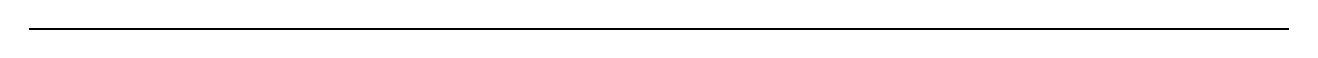
\begin{tikzpicture}
        \draw[thick] (-6.5,0)--(9.5,0);
    \end{tikzpicture}
\end{center}

\setcounter{section}{0}
\section{Preguntas y actividades}
\begin{enumerate}
    \item \textbf{Preguntas}
    Y sus respuestas
    \item \textbf{Actividades}
    Y sus respuestas
\end{enumerate}

\section{Problemas}
\begin{tcolorbox}[title=problema 1]
Descripción del problema
\end{tcolorbox}
Argumentos adecuados
\begin{equation}
    \oint formulas\,\,elementales
\end{equation}
Y más argumentos
\begin{equation*}
    \therefore\,resultado
\end{equation*}
\end{document}
